% \NeedsTeXFormat{LaTeX2e}
\documentclass[12pt,letterpaper]{article}
\usepackage[spanish]{babel}
\usepackage[ansinew]{inputenc}
\usepackage[right=2cm,left=2cm,top=3cm,bottom=3cm,headsep=1cm,footskip=0.5cm]{geometry}
\usepackage[dvips]{graphicx}
\usepackage[nobib]{CoverPage}
\usepackage{invoice}
\usepackage{pifont}
\usepackage{xcolor}

\usepackage[T1]{fontenc} % recommended for languages with accents
% \usepackage[utf8]{inputenc}
\usepackage[latin1]{inputenc}

\usepackage[hidelinks]{hyperref}
\hypersetup{colorlinks=false}

\usepackage{fontspec}
\usepackage[misc]{ifsym}


% Awesome fonts
\usepackage{fontawesome}
% \newfontfamily{\FA}{FontAwesome Regular}
% \def\twitter{{\FA \faTwitter}}
% \usepackage[hidelinks,linkbordercolor=false]{hyperref}
% \hypersetup{
% 	colorlinks{false}
% 	urlcolor{magenta}
% 	filecolor{cyan}
% 	linkcolor{blue}
% 	linkbordercolor{false}
% 	colorlinks{false}
% }

% lscape.sty Produce landscape pages in a (mainly) portrait document.
%\usepackage{lscape}

%\usepackage{rotating} % To display tables in landscape

\usepackage[paper=portrait,pagesize]{typearea} % 


% NOTE Trying Fancy tables

\usepackage[usenames,dvipsnames]{xcolor}
\usepackage{tcolorbox}
\usepackage{tabularx}
\usepackage{array}
\usepackage{colortbl}
\tcbuselibrary{skins}

\newcolumntype{Y}{>{\raggedleft\arraybackslash}X}

\tcbset{tab1/.style={fonttitle=\bfseries\large,fontupper=\normalsize\sffamily,
colback=yellow!10!white,colframe=red!75!black,colbacktitle=Salmon!40!white,
coltitle=black,center title,freelance,frame code={
\foreach \n in {north east,north west,south east,south west}
{\path [fill=red!75!black] (interior.\n) circle (3mm); };},}}

\tcbset{tab2/.style={enhanced,fonttitle=\bfseries,fontupper=\normalsize\sffamily,
colback=yellow!10!white,colframe=red!50!black,colbacktitle=Salmon!40!white,
coltitle=black,center title}}

%% Fancy tables

%%% Trying Fancy Background Image 
\usepackage{transparent}
\usepackage{eso-pic}
\newcommand\BackgroundPic{%
\put(0,0){%
\parbox[b][\paperheight]{\paperwidth}{%
\vfill
\centering
%{\transparent{0.4} 
\includegraphics[width=\paperwidth,height=\paperheight,keepaspectratio,clip]{img/background.png}}\vfill
{\transparent{0.4} 
\includegraphics[width=\paperwidth,height=\paperheight,clip]{img/background.png}}\vfill
}}}
%%% End Trying Fancy Background Image


\usepackage{pstricks}
\usepackage{pst-all}

\newpsobject{malla}{psgrid}{subgriddiv=1,griddots=10,gridlabels=6pt}

% for quotes
% \usepackage{csquotes}

% \usepackage{pstcol} % para color
% \usepackage{pst-node} % para diagramas
% \usepackage{pst-plot} % para representacion de datos
% funciones, etc


\usepackage{tocloft}
%%gmedina solution
\renewcommand{\listfigurename}{Imagenes}
\renewcommand{\listtablename}{Tablas}
\renewcommand{\contentsname}{Contenidos}

\renewcommand{\figurename}{Imagen}
\renewcommand{\tablename}{Datos}



\newcommand{\listequationsname}{Equaciones}
\newlistof{myequations}{equ}{\listequationsname}
\newcommand{\myequations}[1]{%
\addcontentsline{equ}{myequations}{\protect\numberline{\theequation}#1}\par}
\setlength{\cftmyequationsnumwidth}{2.5em}% Width of equation number in List of Equations


 \usepackage{marvosym} % telephoneicons



\usepackage{mathtools}

\usepackage{verbatim}
\usepackage{listings}
% \usepackage{color}
% \lstset{language=PHP}
% \lstset{basicstyle=\ttfamily,
%  showstringspaces=false,
%  commentstyle=\color{red},
%  keywordstyle=\color{blue}
% }
% \usepackage{listings}
% \usepackage{color}





\usepackage{fancyheadings}
% This defines some new pagestyles which you can invoke with:
% \pagestyle{fancy}
% or
\pagestyle{fancyplain}
\newcommand{\tstamp}{\today}
\renewcommand{\chaptermark}[1]{\markboth{#1}{}}
\renewcommand{\sectionmark}[1]{\markright{#1}}
\lhead[\fancyplain{}{\thepage}]         {\fancyplain{}{\rightmark}}
\chead[\fancyplain{}{}]                 {\fancyplain{}{}}
\rhead[\fancyplain{}{\rightmark}]       {\fancyplain{}{\thepage}}
\lfoot[\fancyplain{}{}]                 {\fancyplain{\tstamp}{\tstamp}}
\cfoot[\fancyplain{\thepage}{}]         {\fancyplain{\thepage}{}}
\rfoot[\fancyplain{\tstamp} {\tstamp}]  {\fancyplain{}{}}





\definecolor{mygreen}{rgb}{0,0.6,0}
\definecolor{mygray}{rgb}{0.5,0.5,0.5}
\definecolor{mymauve}{rgb}{0.58,0,0.82}
\definecolor{kblue}{HTML}{2882EE}
\definecolor{kgreen}{HTML}{3F4DF5}
\definecolor{oblue}{HTML}{112ADE}
\definecolor{kgray}{HTML}{3A3A3A}
\definecolor{alert}{HTML}{C21B4D}
\definecolor{blackgreen}{HTML}{687170}
\definecolor{asome}{HTML}{22a3db}
\definecolor{kblues}{HTML}{1a5599}
\definecolor{ktext}{HTML}{0f2b6c}

%687170
% \lstset{ %
%   backgroundcolor=\color{white},   % choose the background color; you must add \usepackage{color} or \usepackage{xcolor}
%   basicstyle=\footnotesize,        % the size of the fonts that are used for the code
%   breakatwhitespace=false,         % sets if automatic breaks should only happen at whitespace
%   breaklines=true,                 % sets automatic line breaking
%   captionpos=b,                    % sets the caption-position to bottom
%   commentstyle=\color{mygreen},    % comment style
%   deletekeywords={...},            % if you want to delete keywords from the given language
%   escapeinside={\%*}{*)},          % if you want to add LaTeX within your code
%   extendedchars=true,              % lets you use non-ASCII characters; for 8-bits encodings only, does not work with UTF-8
%   frame=single,	                   % adds a frame around the code
%   keepspaces=true,                 % keeps spaces in text, useful for keeping indentation of code (possibly needs columns=flexible)
%   keywordstyle=\color{blue},       % keyword style
%   language=Octave,                 % the language of the code
%   otherkeywords={*,...},            % if you want to add more keywords to the set
%   numbers=left,                    % where to put the line-numbers; possible values are (none, left, right)
%   numbersep=5pt,                   % how far the line-numbers are from the code
%   numberstyle=\tiny\color{mygray}, % the style that is used for the line-numbers
%   rulecolor=\color{black},         % if not set, the frame-color may be changed on line-breaks within not-black text (e.g. comments (green here))
%   showspaces=false,                % show spaces everywhere adding particular underscores; it overrides 'showstringspaces'
%   showstringspaces=false,          % underline spaces within strings only
%   showtabs=false,                  % show tabs within strings adding particular underscores
%   stepnumber=2,                    % the step between two line-numbers. If it's 1, each line will be numbered
%   stringstyle=\color{mymauve},     % string literal style
%   tabsize=2,	                   % sets default tabsize to 2 spaces
%   title=\lstname                   % show the filename of files included with \lstinputlisting; also try caption instead of title
% }


\lstdefinestyle{customc}{
  belowcaptionskip=1\baselineskip,
  breaklines=true,
  frame=L,
  xleftmargin=\parindent,
  language=PHP,
  showstringspaces=false,
  basicstyle=\footnotesize\ttfamily,
  keywordstyle=\bfseries\color{blue!40!black},
  commentstyle=\itshape\color{mymauve!40!black},
  identifierstyle=\color{blue},
  stringstyle=\color{mygreen},
  numberstyle=\tiny\color{mygray},
}

%-----------------------------------------------------------------------
% after parsing the BibTeX data and reading the "CoverPage.cfg"
% config file, you can manually setup the cover main in your main
% document:
% \emph{elephantom.soporte@gmail.com}
\CoverPageSetup{title=Desarrollo de Sistemas,author=Cyberia,institute={\copyright{Cyberia}},insource={\href{mailto:cybberio@gmail.com}{\faEnvelopeO\ \emph{cybberio@gmail.com }} \\ \href{https://www.devs.com.mx}{\faExternalLink\ \emph{devs.com.mx}} },copyright={\copyright{Cyberia} } }
% \CoverPageSetup{institute=C,insource=D,copyright=E}
% this line would create an automatic IEEE copyright notice
\CoverPageSetup{year=2020,publisher=Cyberio}
% \CoverPageSetup{year=2017,publisher=IEEE}
% and settings like this set the source; booktitle would also work
% \CoverPageSetup{journal=\textit{El sistema se divide en cuatro m\'odulos, un sistema de logueo y un historial de procesos}}
% Of course, all necessary keys can be combined in a single
% \CoverPageSetup command.

% \CoverPageSetup{institute = {Institute of Applied Computer Science}}
% \renewcommand{\CoverPageHeader}{%
% \includegraphics[width=\textwidth]{img/elephantom_transparent.png}
% }

\renewcommand{\CoverPageHeader}{%
%  {\includegraphics[width=.20\textwidth]{geonext.png}}%
  {
  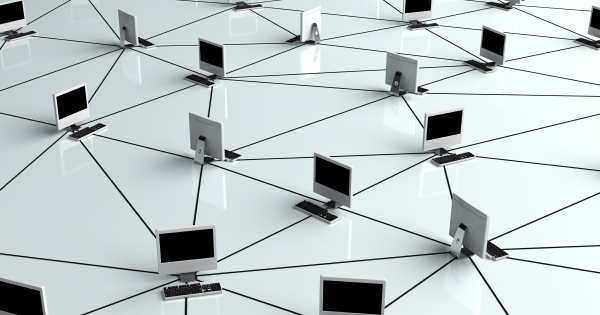
\includegraphics[width=180mm]{img/nas_net.jpg}}%
  }
  % \LARGE\bfseries%
  % \hrulefill{} {\color{green}HEADER LOGO} \hrulefill}
% \renewcommand{\CoverPageFooterLogo}{%
%   \Huge\sffamily%
%   {\color{blue}L-O-G-O}}
% \renewcommand{\CoverPageBody}{\includegraphics[width=.35\textwidth]{rwthlogo}}
% \renewcommand{\CoverPageFooter}{\includegraphics[width=.35\textwidth]{rwthlogo}}

\renewcommand{\CoverPageFooterLogo}{
\includegraphics[width=.15\textwidth]{img/cyberia.jpg}}
%-----------------------------------------------------------------------
\begin{document}
  \AddToShipoutPicture{\BackgroundPic}
  {
	\sffamily % Start the Document
	% for smallcaps shape use the command \scshape
	\title{Propuesta de Desarrollo}
	\author{\copyright Cyberia}
	\maketitle
	\tableofcontents
	% \listoffigures
	% \listofmyequations
	%   \makeglossaries
	\newpage
  }




%\newpage

% \newpage
%   \begin{section}{\color{kblue}\sffamily{Add Document}}
%   \sffamily
%   {
%
%   }
%   \end{section}



% FOR FOOTNOTES
  % \footnotesize{\scshape{}}

% FOR TABLES
% \begin{table}
% \end{table}

% EQUATIONS
% \begin{equation}
% 	costoLlamada = { totalDeMinutos x tarifa[codigoDePais] }
% 	\label{eq:costo de la llamada}
% \end{equation}
%
% \myequations{costo_call}


\newpage
\KOMAoptions{paper=portrait,pagesize}
\begin{section}{\color{kblue}\sffamily{Proyecto Edi-q}}
  \sffamily{




      \begin{figure}[htb]
        \centering
        
\includegraphics[angle=0,width=0.5\textwidth]{img/edi-q.jpg}
	\caption{\href{https://www.ediq.mx}{\faExternalLink\ \emph{Edi-q}}}
        \label{sel064}
      \end{figure}
  }
\end{section}


\newpage
\KOMAoptions{paper=portrait,pagesize}
\begin{section}{\color{kblue}\sffamily{Objetivo General}}
  \sffamily{
\begin{itemize}
    \bigskip
	\bigskip
		\item Diseñar e Implementar una interfaz permita utilizar los libros de texto de digitalizados de ediq como si se tratasen de los libros reales
		\item La interfaz debe permitir escribir las respuestas en los campos del libro digitalizado 
		\item Conservar la estructura del libro en su totalidad ,Colores,Diseño, Tipografías , etc.
		\item El Desarrollo debe ser Independiente y capaz de integrarse con el Desarrollo actual
		\item Debe Integrar modulos para Administracion de calificaciones de alumnos

		\smallskip
		Nuestra prioridad es construir una relación comercial optima, que permita  el crecimiento de nuestro cliente y de la sociedad realizada.
		\smallskip
		
	

\end{itemize}

 }
  \end{section}
%      \begin{figure}[htb]
%        \centering
%        
\includegraphics[angle=0,width=0.5\textwidth]{img/edi-q.jpg}
%        \caption{DS}
%        \label{sel064}
%      \end{figure}
\newpage
\KOMAoptions{paper=portrait,pagesize}
\begin{section}{\color{kblue}\sffamily{Planteamiento}}
  \sffamily{
\begin{itemize}
	\item Agregar nuevas caracteristicas que permitan la interaccion con los libros digitalizados de la plataforma 
	\item Integrar o Crear un módulo para Administrar la información generada (Calificaciones,Maestros,Alumnos) 
	\item Integrar o Crear un módulo que evalue las Actividades de manera automatizada
	\item Integrar o Crear un módulo que presente los resultados con los indicadores mas importantes (Dashboard)

\end{itemize}


  \end{section}



\newpage
\KOMAoptions{paper=portrait,pagesize}
\begin{section}{\color{kblue}\sffamily{Alcances del Proyecto}}
  \sffamily{
\begin{itemize}
	\item Interfaz que Simulara el uso natural de un libro 
	\item Capacidad de responder los ejercicios sobre el libro digital 
	\item Automatizacion del proceso de evaluación de los alumnos que realicen actividades en la plataforma digital
	\item Administración y precentación de la información procedente de los alumnos en tiempo real (Dashboard)
	

\end{itemize}

%      \begin{invoice}{MXN}{16}
%	    \ProjectTitle{\color{red}Relacion de Montos}%
%            \Fees{Proveedor}
%            \Fee{Poly,TBO7911166Z6,Poliza}{16000}{1}
%            \Fee{Poly,TBO7911166Z6,Val y Resg. de Fac.}{2}{1300}
%            \Fee{HugoCid,TBO7911166Z6,Mon.redes}{38500}{1}
%            \Fee{HugoCid,TLO970502AA4,Imp. y dev. de software}{50166.67}{1}
% 	    \Discount{}{2000}
%      \end{invoice}
%


%ImG
\newpage

%\href[options]{URL}{text}

   \href{https://baizabal.xyz/demos}{\faExternalLink\ \emph{Prueba en linea}}


      \begin{figure}[htb]
        \centering
        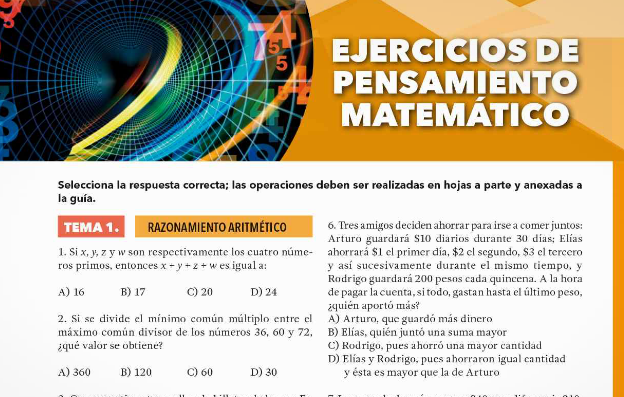
\includegraphics[angle=0,width=75mm,height=50mm]{img/libro_orig.png}
        \caption{hoja Original}
        \label{sel064}
      \end{figure}

      \begin{figure}[htb]
        \centering
        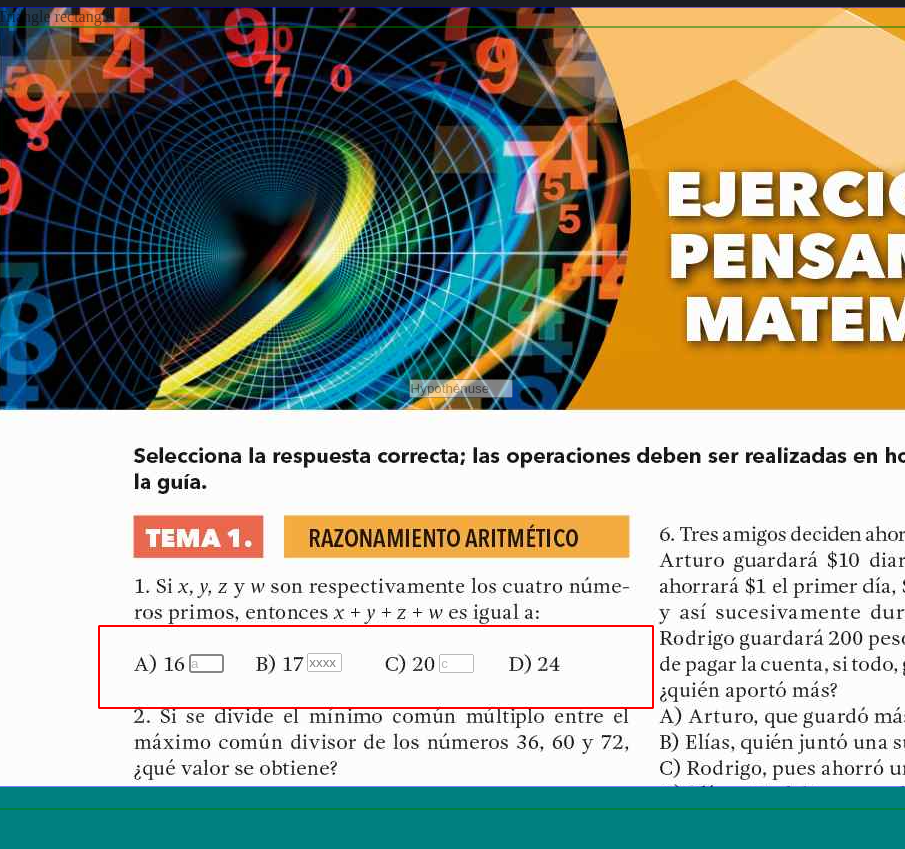
\includegraphics[angle=0,width=65mm,height=50mm]{img/libro.png}
	\caption{Prueba de concepto} 
        \label{sel064}
      \end{figure}


%live demo

%https://baizabal.xyz/demos/












 }
  \end{section}







  
%  \begin{section}{\color{kblue}\sffamily{link}}
%    \sffamily
%    {
% 	\begin{figure}[htb]
%		    \centering
%		    \includegraphics[angle=0,width=80mm]{img/link.jpg}
%		    \caption{..,}
%		    \label{dc7600}
%	\end{figure} 

%    }
%  \end{section}
  

%\newpage
%\KOMAoptions{paper=portrait,pagesize}
%\begin{section}{\color{kblue}\sffamily{Consideraciones}}
%  \sffamily{
%\begin{itemize}
%        \item Al adquirir nuestros servicios se agrega una capa de cifrado a la transferencia de data, adicional a la proporcionada por los protocolos locales del servidor en la nube.
%		\item El acceso a los servidores será administrado por el área de TI de la empresa contratante (GST), teniendo a su disposición todos los recursos del servicio contratado.
%		\item La frecuencia de respaldo de datos será determinada y supervisada por el área de TI de la empresa contratante (GST).
%		\item El servicio en la nube cuenta con una amplia capacidad para soportar los diferentes sistemas base (Windows, Linux, Unix).
%		\item Se integra una p\'oliza de mantenimiento, que asegura un \'optimo aprovechamiento de los recursos contratados (se har\'a una notificaci\'on con no menos de 24 hrs. de anticipaci\'on).
%		\item Se integran 2 modelos de trabajo en base al pago: mensualidad y anualidad. El pago mensual se establece en base al primer pago. La anualidad integra un descuento por 1 mes al pagar en esta modalidad.
%		\item Con SIE olv\'idate de los cargos ocultos por tasas de transferencia, el pago definido mensual o anual no sufre modificaciones.
%		\item La p\'oliza de mantenimiento incluye apoyo t\'ecnico con los servicios instalados en el servdidor.
%		\item Para finalizar la relación comercial, se debe realizar la notificaci\'on 30 d\'ias antes, dentro de un periodo de p\'oliza vigente.
%\end{itemize}
%
% }
%  \end{section}
%      \begin{figure}[htb]
%        \centering
%        \includegraphics[angle=0,width=90mm,height=45mm]{img/iOT.jpg}
%        \caption{Tiempos}
%        \label{sel064}
%      \end{figure}
%

\newpage
\KOMAoptions{paper=portrait,pagesize} % shiwcth to lanscape

  \begin{section}{\color{kblue}\sffamily{Propuesta Económica}}
    \sffamily
    {




\begin{tcolorbox}[
		  tab2,
		  tabularx={l||c||r},
		  title=Propuesta Economica,
		  boxrule=0.5pt,
		  colframe=cyan!50!black,
		  colbacktitle=kblues,
		  coltitle=white,
		  colback=white,
		  colupper=ktext
		]
  \textbf {Propuesta 1}		  & \textbf{Descripción}  & \textbf{Total}	\\\hline\hline
  Tiempo de Desarrollo		  & 6 meses		  &			\\\hline\hline % <--  \\\hline\hline
  Anticipo del 50\%		  &			  &			\\\hline\hline % <--  \\\hline\hline
  Primer Pago del 25\%		  &			  &			\\\hline\hline % <--  \\\hline\hline
  Segundo y último Pago del 25\%  &			  &			\\\hline\hline % <--  \\\hline\hline
				  &			  & \$182,000.\textsuperscript{00}      	\\\hline\hline % <--  \\\hline\hline


\end{tcolorbox}


\begin{tcolorbox}[
		  tab2,
		  tabularx={l||c||r},
		  title=Propuesta Economica,
		  boxrule=0.5pt,
		  colframe=cyan!50!black,
		  colbacktitle=kblues,
		  coltitle=white,
		  colback=white,
		  colupper=ktext
		]
  \textbf {Propuesta 2}		  & \textbf{Descripción}  & \textbf{Total}	\\\hline\hline
  Tiempo de Desarrollo		  & 9 meses		  &			\\\hline\hline 
  Equipo de Desarrolladores\%     & 2 desarrolladores	  &			\\\hline\hline 
  Pago Mensual 		          & \$9,000.\textsuperscript{00} & \$18,000.\textsuperscript{00} \\\hline\hline 
				  &			  & \$162,000.\textsuperscript{00}  \\\hline\hline


\end{tcolorbox}




\begin{tcolorbox}[
		  tab2,
		  tabularx={l||c||r},
		  title=Propuesta Economica,
		  boxrule=0.5pt,
		  colframe=cyan!50!black,
		  colbacktitle=kblues,
		  coltitle=white,
		  colback=white,
		  colupper=ktext
		]
  \textbf {Propuesta 3}		  & \textbf{Descripción}  & \textbf{Total}	\\\hline\hline
  Tiempo de Desarrollo		  & 18 meses		  &			\\\hline\hline 
  Equipo de Desarrolladores\%     & 2 desarrolladores	  &			\\\hline\hline 
  Pago Mensual 		          & \$6,055.\textsuperscript{00} & \$12,110.\textsuperscript{00} \\\hline\hline 
				  &			  & \$272,980.\textsuperscript{00}  \\\hline\hline


\end{tcolorbox}

%
% \begin{itemize}
%	\item \textbf {Pago mensual:} SIN CONTRATO FORZOSO  (la cancelación se debe realizar la notificaci\'on 30 d\'ias antes, dentro de un periodo de p\'oliza vigente.)
%\end{itemize}

    }
  \end{section}
 
\newpage
\KOMAoptions{paper=portrait,pagesize}
\begin{section}{\color{kblue}\sffamily{Firma de conformidad}}
  \sffamily{
\begin{itemize}
\bigskip
\bigskip
    \item Propuesta\:\ \ \ \ \ \underline {}\ \ \ \ \ \ \ \ \underline{}
\bigskip
\bigskip
    \item Nombre\:\ Quimico. ? 
	\medskip
	\item Firma\: \_\_\_\_\_\_\_\_\_\_\_\_\_\_\_\_\_\_\_\_\_ 
\bigskip
    \item Nombre\:\ Ing. Carlos 
	\medskip
	\item Firma\: \_\_\_\_\_\_\_\_\_\_\_\_\_\_\_\_\_\_\_\_\_ 
\bigskip
	\item Nombre\:\ Ing. Jesús A. Mendoza Baizabal
    \medskip
	\item Firma\: \_\_\_\_\_\_\_\_\_\_\_\_\_\_\_\_\_\_\_\_\_
\end{itemize}

 }
  \end{section}


\end{document}
